\documentclass[14pt,fleqn]{extarticle}
\RequirePackage{prepwell}

\previewoff 

\begin{document} 
\begin{snippet}
    \correct
    
    The figure below shows an ellipse and a circle inside it. 
    $A = (0,1), B = (1,0)$ and $C = (2,0)$ 
    
    \begin{center}
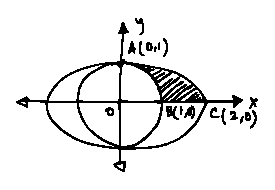
\includegraphics[scale=0.3]{figure.eps}
\end{center}

The shaded portion can therefore be described as 
\small\[ \left\lbrace (x,y) : \cos\theta \leq x \leq 2\cos\theta, y = \sin\theta, \theta \in \left(0,\frac\pi{2}  \right)\right\rbrace\]\normalsize
    
    \reason
    
    We have two curves in the figure -- an ellipse and a circle 
    
    \begin{center}
  \begin{tabular}{NNl}
   \toprule
        y & x & Curve   \\
   \midrule 
   \sin\theta & 2\cos\theta & Ellipse \\
   \midrule 
   \sin\theta & \cos\theta & Circle \\
    \bottomrule
  \end{tabular}
\end{center}

The conditions have been given to us in set-builder form. 
And taken together, they mean the following 

\begin{center}
  \begin{tabular}{Nl}
   \toprule
        \text{Condition} & Meaning  \\
   \midrule 
   x \leq 2\cos\theta,y =  \sin\theta & Inside the ellipse \\ 
    \midrule 
    x\geq \cos\theta, y = \sin\theta & Outside the circle \\
    \midrule 
    0\leq \theta\leq \frac\pi{2} & First quadrant only \\
    \bottomrule
  \end{tabular}
\end{center}

Which are points in the shaded region 
    
\end{snippet} 
\end{document} 